\chapter{逻辑设计}
\thispagestyle{empty}
\section{E-R图向关系模型的转变}
\subsection{实体集模式}
\subsubsection{模式设计}
通过转换上述实体集,我们可以得到表\ref{tab:entityschema}中的实体集模式:
\begin{table}[!hpt]
    \caption{实体集模式}
    \label{tab:entityschema}
    \centering
    \begin{tabular}{l} \toprule
         \textit{bike}(\textit{\underline{bike\_ID},production\_date,coordinate,battery\_ramaining\_capacity})\\
         \textit{bike\_status}(\textit{\underline{bike\_ID},\underline{status}})\\
         \textit{usage}(\textit{\underline{bike\_ID},\underline{time},coordinate,action})\\
         \textit{parking\_area}(\textit{\underline{parking\_area\_ID},name,coordinate,radius})\\
         \textit{scheduling}(\textit{\underline{bike\_ID},\underline{time},coordinate,action})\\
         \textit{to\_be\_reviewed}(\textit{\underline{bike\_ID},\underline{time}})\\
         \textit{to\_be\_reviewed\_status}(\textit{\underline{bike\_ID},\underline{time},\underline{status}})\\
         \textit{to\_be\_reviewed\_proof\_material}(\textit{\underline{bike\_ID},\underline{time},\underline{no},proof\_material})\\\bottomrule
    \end{tabular}
  \end{table}

  在转换过程中,我们认为坐标、日期以及时间都是不可分割的单元。在实际应用场景中,也常常将它们作为整体来进行使用。

  对于弱实体集\textit{usage,scheduling}和\textit{to\_be\_reviewed},它们的模式的主码由自身的识别器\textit{time}和
  识别集的主码组成。

  对于实体集\textit{bike}中的属性\textit{status}和实体集\textit{to\_be\_reviewed}中的属性\textit{status}和\textit{proof\_material},它们是多值属性。
  为此,转换为模式时,额外创建模式\textit{bike\_status,to\_be\_reviewed\_status},\textit{to\_be\_}\\\textit{reviewed\_proof\_material}。
  模式\textit{bike\_status,to\_be\_reviewed\_status}的属性由原实集的主码和对应的多值属性组合而成,并且以它们作为主码。
  由于我们假设调度员可能会由于操作失误而上传多张相同的图片,同时,为了避免以图片数据作为主码的一部分,我们在模式\textit{to\_be\_reviewed\_proof\_material}中添加了\textit{no}域,用于表示证明材料的编号,并与
  \textit{bike\_ID,time}一同作为该模式的主码。
  
  对于其余强实体集,它们的模式的主码和属性与原来保持一致。

  \subsubsection{属性类型设计}
图\ref{tab:tobereviewedstatus}-\ref{tab:tobereviewedproofmaterial}为各实体集模式中属性的类型。
各类型定义与PostgreSQL文档\cite{data}一致。其中,\textbf{status}为自定义的枚举类型。

\begin{figure}[!htp]
    \begin{minipage}{0.33\textwidth}
      \centering
      \caption{\textit{to\_be\_reviewed\_status}属性类型}
      \label{tab:tobereviewedstatus}
      \begin{tabular}{ll}\toprule
        属性&类型\\\midrule
       \textit{bike\_ID}&\textbf{char}(20)\\
       \textit{time}&\textbf{timestamp}\\
       \textit{status}&\textbf{status}\\
       \bottomrule
      \end{tabular}



    \end{minipage}\hfill
    \begin{minipage}{0.33\textwidth}
      \centering
      \caption{\textit{bike\_status}属性类型}
      \label{tab:bikestatus}
      \begin{tabular}{ll}\toprule
        属性&类型\\\midrule
       \textit{bike\_ID}&\textbf{char}(20)\\
       \textit{status}&\textbf{status}\\
       \bottomrule
      \end{tabular}
    \end{minipage}\hfill
    \begin{minipage}{0.33\textwidth}
      \centering
      \caption{\textit{usage}属性类型}
      \label{tab:usage}
      \begin{tabular}{ll}\toprule
        属性&类型\\\midrule
       \textit{bike\_ID}&\textbf{char}(20)\\
       \textit{time}&\textbf{timestamp}\\
       \textit{coordinate}&\textbf{point}\\
       \textit{action}&\textbf{boolean}\\
       \bottomrule
      \end{tabular}
    \end{minipage}\hfill
  \end{figure}

\begin{figure}[!htp]
    \begin{minipage}{0.33\textwidth}
      \centering
      \caption{\textit{parking\_area}属性类型}
      \label{tab:parkingarea}
      \begin{tabular}{ll}\toprule
        属性&类型\\\midrule
       \textit{parking\_area\_ID}&\textbf{serial}\\
       \textit{name}&\textbf{char}(20)\\
       \textit{coordinate}&\textbf{point}\\
       \textit{radius}&\textbf{real}\\
       \bottomrule
      \end{tabular}
    \end{minipage}\hfill
    \begin{minipage}{0.33\textwidth}
      \centering
      \caption{\textit{scheduling}属性类型}
      \label{tab:scheduling}
      \begin{tabular}{ll}\toprule
        属性&类型\\\midrule
       \textit{bike\_ID}&\textbf{char}(20)\\
       \textit{time}&\textbf{timestamp}\\
       \textit{coordinate}&\textbf{point}\\
       \textit{action}&\textbf{boolean}\\
       \bottomrule
      \end{tabular}
    \end{minipage}\hfill
    \begin{minipage}{0.33\textwidth}
      \centering
      \caption{\textit{to\_be\_reviewed}属性类型}
      \label{tab:tobereviewed}
      \begin{tabular}{ll}\toprule
        属性&类型\\\midrule
       \textit{bike\_ID}&\textbf{char}(20)\\
       \textit{time}&\textbf{timestamp}\\
       \bottomrule
      \end{tabular}
    \end{minipage}\hfill
  \end{figure}

\begin{figure}[!htp]
    \begin{minipage}{0.5\textwidth}
      \centering

      \caption{\textit{bike}属性类型}
      \label{tab:bike}
      \begin{tabular}{ll}\toprule
        属性&类型\\\midrule
       \textit{bike\_ID}&\textbf{char}(20)\\
       \textit{production\_date}&\textbf{date}\\
       \textit{coordinate}&\textbf{point}\\
       \textit{battery\_remaining\_capacity}&\textbf{real}\\
       \bottomrule
      \end{tabular}

    \end{minipage}\hfill
    \begin{minipage}{0.5\textwidth}
      \centering
      \caption{\textit{to\_be\_reviewed\_proof\_material}属性类型}
      \label{tab:tobereviewedproofmaterial}
      \begin{tabular}{ll}\toprule
        属性&类型\\\midrule
       \textit{bike\_ID}&\textbf{char}(20)\\
       \textit{time}&\textbf{timestamp}\\
       \textit{no}&\textbf{smallint}\\
       \textit{proof\_material}&\textbf{text}\\
       \bottomrule
      \end{tabular}
    \end{minipage}\hfill
  \end{figure}
\subsection{关系集模式}
\subsubsection{模式设计}
  通过转换上述关系集,我们可以得到表\ref{tab:relationschema}中的关系集模式:

  \begin{table}[!hpt]
      \caption{关系集模式}
      \label{tab:relationschema}
      \centering
      \begin{tabular}{l} \toprule
           \textit{contain}(\textit{\underline{bike\_ID},\underline{parking\_area\_ID}})\\
           \bottomrule
      \end{tabular}
    \end{table}

    在转换的过程中,联系弱实体集和其对应识别集的关系集\textit{bike\_usage,bike\_scheduling}和\textit{bike\_to\_be\_reviewed}被略去,因为这是冗余的\cite{dbconcept2}。

    关系集\textit{contain}为“多对多”的二元关系集,其模式的主码由它关联起来的实体集模式的主码组合而成。

\subsubsection{属性类型设计}
  关系集模式中属性的类型与实体集中的相应属性类型保持一致。图\ref{tab:contain}为\textit{contain}模式中属性的类型。
  \begin{figure}[!htp]
      \centering
      \caption{\textit{contain}属性类型}
      \label{tab:contain}
      \begin{tabular}{ll}\toprule
        属性&类型\\\midrule
       \textit{bike\_ID}&\textbf{char}(20)\\
       \textit{parking\_area\_ID}&\textbf{serial}\\
       \bottomrule
      \end{tabular}
\end{figure}
\subsection{约束设计}
图\ref{contraint:bike}-\ref{contraint:tobereviewedproofmaterial}为各模式中的属性所需遵循的约束。

约束设计主要分为两部分:外码约束和其他约束。

\paragraph{外码约束}
外码约束主要有三个来源:

\begin{enumerate}
    \item 关系集转化为关系集模式时所产生的;
    \item 转化复杂类型时所产生的;
    \item 转化弱实体集时所产生的。
\end{enumerate}

在本数据库中,由于多值属性而额外生成的模式\textit{bike\_status,to\_be\_reviewed\_status,to\_be\_}\\\textit{reviewed\_proof\_material}与原模式之间存在外码约束。
它们的主码需引用原模式的主码。

弱实体集\textit{usage,scheduling,to\_be\_reviewed}转换为模式时,需遵循外码约束,引用其识别集的主码。

其余外码约束来自于由关系集\textit{contain}转化而来的关系集模式,需要引用模式\textit{parking\_area}与\textit{bike}的主码。

\paragraph{其他约束}
本数据库中的其他约束包括主码约束(非空且唯一)、非空约束、唯一约束和CHECK约束。

由于本数据库中除了\textit{proof\_material,radius}外的其他所有域理论上都可以由相应的设备自动生成,如电池剩余电量,又或者是必不可少的一部分,例如停车区域半径,所以所有属性都遵循非空约束。

对于坐标、时间戳、证明材料等数据,我们不作唯一约束要求。

在本数据库中,CHECK约束主要用于确保停车区域半径大于一定值,我们假设停车区域半径至少大于10米。

特别地,\textit{text}表中的记录与“违规停车”在语义上有着直接关联。我们规定一辆单车当且仅当不出现在\textit{text}表中时拥有“违规停车”状态。
为了维护该约束,我们采用触发器。

\begin{figure}[!htp]
      \centering
      \caption{\textit{bike}属性约束}
      \label{contraint:bike}
      \begin{tabular}{ll}\toprule
        属性&约束\\\midrule
       \textit{bike\_ID}&\textbf{PRIMIARY KEY}\\
       \textit{production\_date}&\textbf{NOT NULL}\\
       \textit{coordinate}&\textbf{NOT NULL}\\
       \textit{battery\_remaining\_capacity}&\makecell[l]{\textbf{CHECK} \textit{battery\_remaining\_capacity between 0 AND 1}\\\textbf{NOT NULL}}\\
       \bottomrule
      \end{tabular}
\end{figure}

\begin{figure}[!htp]
    \begin{minipage}{0.5\textwidth}
      \centering
      \caption{\textit{to\_be\_reviewed\_status}属性约束}
      \label{contraint:tobereviewedstatus}
      \begin{tabular}{ll}\toprule
        属性&约束\\\midrule
       \textit{bike\_ID}&\textbf{REFERENCES} \textit{bike}\\
       \textit{time}&\\
       \textit{status}&\\
       \textit{(bike\_ID,time,status)}&\textbf{PRIMIARY KEY}\\
       \bottomrule
      \end{tabular}
    \end{minipage}\hfill
    \begin{minipage}{0.5\textwidth}
      \centering
      \caption{\textit{bike\_status}属性约束}
      \label{contraint:bikestatus}
      \begin{tabular}{ll}\toprule
        属性&约束\\\midrule
       \textit{bike\_ID}&\textbf{REFERENCES} \textit{bike}\\
       \textit{status}&\\
       \textit{(bike\_ID,status)}&\textbf{PRIMIARY KEY}\\
       \bottomrule
      \end{tabular}
    \end{minipage}\hfill
 \end{figure}

\begin{figure}[!htp]
    \begin{minipage}{0.5\textwidth}
      \centering
      \caption{\textit{usage}属性约束}
      \label{contraint:usage}
      \begin{tabular}{ll}\toprule
        属性&约束\\\midrule
       \textit{bike\_ID}&\\
       \textit{time}&\\
       \textit{coordinate}&\textbf{NOT NULL}\\
       \textit{action}&\textbf{NOT NULL}\\
       \textit{(bike\_ID,time)}&\textbf{PRIMIARY KEY}\\
       \textit{(bike\_ID,time)}&\textbf{REFERENCES} \textit{bike\_status}\\
       \bottomrule
      \end{tabular}
    \end{minipage}\hfill
    \begin{minipage}{0.5\textwidth}
      \centering
      \caption{\textit{parking\_area}属性约束}
      \label{contraint:parkingarea}
      \begin{tabular}{ll}\toprule
        属性&约束\\\midrule
       \textit{parking\_area\_ID}&\textbf{PRIMIARY KEY}\\
       \textit{name}&\textbf{NOT NULL}\\
       \textit{coordinate}&\textbf{NOT NULL}\\
       \textit{radius}&\makecell[l]{\textbf{CHECK} \textit{radius>=10}\\\textbf{NOT NULL}}\\
       \bottomrule
      \end{tabular}
    \end{minipage}\hfill
 \end{figure}


\begin{figure}[!htp]
      \centering
      \caption{\textit{contain}属性约束}
      \label{contraint:contain}
      \begin{tabular}{ll}\toprule
        属性&约束\\\midrule
       \textit{bike\_ID}&\textbf{REFERENCES} \textit{bike}\\
       \textit{parking\_area\_ID}&\textbf{REFERENCES} \textit{parking\_area}\\
       \textit{(bike\_ID,parking\_area\_ID)}&\textbf{PRIMIARY KEY}\\
       \bottomrule
      \end{tabular}
\end{figure}

\begin{figure}[!htp]
    \begin{minipage}{0.5\textwidth}
      \centering
      \caption{\textit{scheduling}属性约束}
      \label{contraint:scheduling}
      \begin{tabular}{ll}\toprule
        属性&约束\\\midrule
       \textit{bike\_ID}&\textbf{REFERENCES} \textit{bike}\\
       \textit{time}&\\
       \textit{coordinate}&\textbf{NOT NULL}\\
       \textit{action}&\textbf{NOT NULL}\\
       \textit{(bike\_ID,time)}&\textbf{PRIMIARY KEY}\\
       \bottomrule
      \end{tabular}
    \end{minipage}\hfill
    \begin{minipage}{0.5\textwidth}
      \centering
      \caption{\textit{to\_be\_reviewed}属性约束}
      \label{contraint:tobereviewed}
      \begin{tabular}{ll}\toprule
        属性&约束\\\midrule
       \textit{bike\_ID}&\textbf{REFERENCES} \textit{bike}\\
       \textit{time}&\\
       \textit{(bike\_ID,time)}&\textbf{PRIMIARY KEY}\\
       \bottomrule
      \end{tabular}
    \end{minipage}\hfill
\end{figure}


\begin{figure}[!htp]

      \centering
      \caption{\textit{to\_be\_reviewed\_proof\_material}属性约束}
      \label{contraint:tobereviewedproofmaterial}
      \begin{tabular}{ll}\toprule
        属性&约束\\\midrule
       \textit{bike\_ID}&\\
       \textit{time}&\\
       \textit{no}&\textbf{CHECK} no>=0\\
       \textit{proof\_material}&\textbf{NOT NULL}\\
       \textit{(bike\_ID,time,no)}&\textbf{PRIMIARY KEY}\\
       \textit{(bike\_ID,status)}&\textbf{REFERENCES} \textit{bike\_status}\\
       \bottomrule
      \end{tabular}

\end{figure}

\subsection{模式图}

图\ref{schema}为本系统所用数据库的模式图。

\begin{figure}[!htbp]
    \centering
    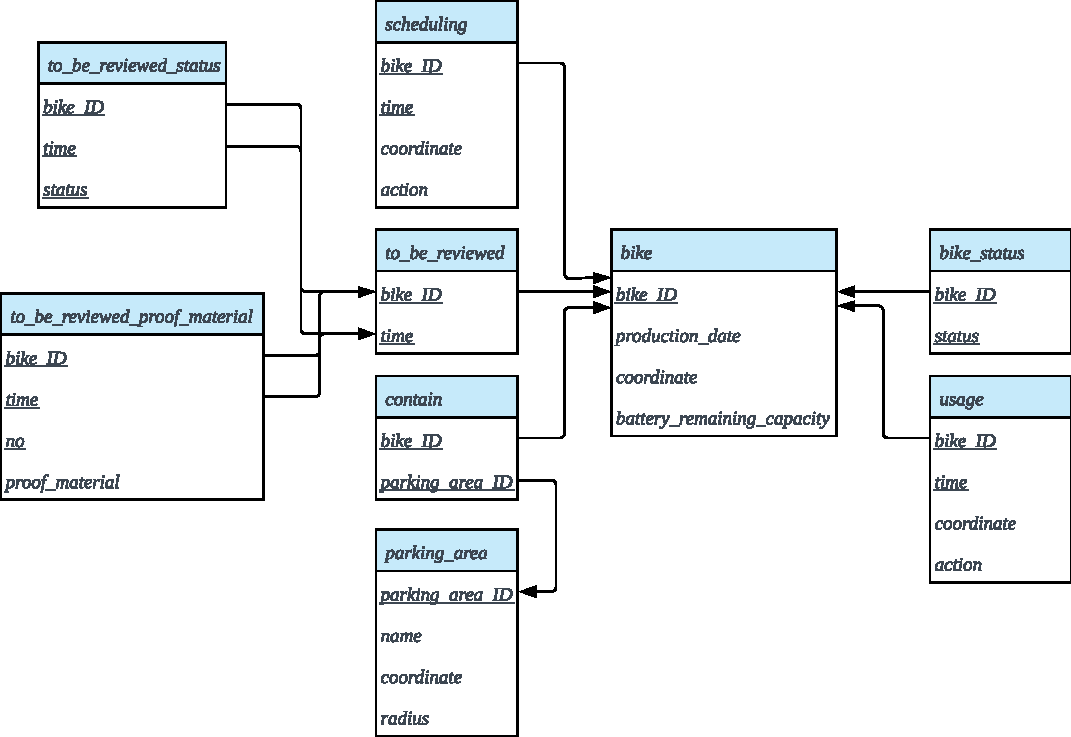
\includegraphics[width=\textwidth]{figures/schema.pdf}
    \caption{模式图}\label{schema}
\end{figure}

\section{数据模型的优化及规范化设计}

\subsection{第一范式}
在从E-R图转换至模式的过程中,我已经将复杂属性拆分开来,所以所有模式满足第一范式。
\subsection{第二范式}
\begin{table}[!hpt]
  \caption{各模式中的函数依赖的正则覆盖}
  \label{tab:functiondependency}
  \centering
  \begin{tabular}{l} \toprule
      $FC_{scheduling}=\{\{bike\_ID,time\}\rightarrow \{coordinate,action\}\}$\\
      $FC_{to\_be\_reviewed}=\varnothing$\\
      $FC_{contain}=\varnothing$\\
      $FC_{parking\_area}=\{parking\_area\_ID\rightarrow \{name,coordinate,radius\}\}$\\
      $FC_{bike}=\{bike\_ID\rightarrow \{production\_date,coordinate,battery\_remaining\_capacity \}\}$\\
      $FC_{to\_be\_reviewed\_proof\_material}=\{\{bike\_ID,time,no\}\rightarrow proof\_material\}$\\
      $FC_{to\_be\_reviewed\_status}=\varnothing$\\
      $FC_{bike\_status}=\varnothing$\\
      $FC_{usage}=\{\{bike\_ID,time\}\rightarrow\{coordinate,action\}\}$\\
       \bottomrule
  \end{tabular}
\end{table}

经过验证,各个模式中不存在部分函数依赖,即所有模式满足第二范式。
\subsection{第三范式}
经过验证,各个模式中不存在传递依赖的关系,即所有模式满足第三范式。
\subsection{BC范式}
经过验证,所有模式满足BC范式。
